\part*{第4章:積分法}
\addcontentsline{toc}{part}{\texorpdfstring{第4章:積分法}{第4章:積分法}}



\section*{p211-212:1}
\addcontentsline{toc}{section}{\texorpdfstring{p211-212:1}{p211-212:1}}


\begin{tleftbar}
    \begin{proof}
        $f$は区間$I$内の$m$個の点$x = a_1, a_2, \ldots, a_m$でのみ$f(x) \ne 0$であるとする.
        この条件のもとで,
        \[
            M = \max_{1 \leqq k \leqq m} \abs{f(a_k)}
        \]
        と定義する.また任意の分割 $\Delta$ に対して,
        \[
            s(f; \Delta; \xi) = \sum_{k \in K(\Delta)} f(\xi_k) v(I_k)
        \]
        である.ここで、$f(\xi_k) \ne 0$である項は高々$m$個であり,その個数を$m_0$とする.
        このような項のみを考慮すると,リーマン和は次のように表せる:
        \[
            s(f; \Delta; \xi) = \sum_{i=1}^{m_0} f(\xi_{k_i}) v(I_{k_i})
        \]
        ここで,$i = 1, 2, \ldots, m_0$は$f(\xi_k) \ne 0$である区間$ I_{k_i} $を走るものとする.

        次に,先に定義した$M$を用いると,
        \[
            \abs{s(f; \Delta; \xi)} = \abs{\sum_{i=1}^{m_0} f(\xi_{k_i}) v(I_{k_i})} \leqq M \sum_{i=1}^{m_0} v(I_{k_i})
        \]
        を得る.さて,$d(\Delta)$を分割$\Delta$の直径とすると,各区間の体積に関して$ v(I_{k_i}) \leqq d(\Delta)^n $だから,
        \[
            \abs{s(f; \Delta; \xi)} \leqq M \sum_{i=1}^{m_0} d(\Delta)^n = m_0 M d(\Delta)^n
        \]
        となる.ここで,リーマン和に寄与する項は$m_0$個であることを用いた.

        ここで,$d(\Delta) \to 0$ とすると,$d(\Delta)^n \to 0$ であるため,
        \[
            \abs{s(f; \Delta; \xi)} \to 0
        \]
        となる.したがって,$f$は区間$I$上でリーマン積分可能であり,
        \[
            \int_{I} f(x)\, dx = 0.
        \]
    \end{proof}
\end{tleftbar}

\section*{p211-212:2}
\addcontentsline{toc}{section}{\texorpdfstring{p211-212:2}{p211-212:2}}


\begin{tleftbar}
    \begin{proof}
        まず,$f$は$I$上で可積分であることから,任意の$\varepsilon >0$に対して,分割$\Delta$が存在して
        \[
            \abs{s(f; \Delta; \xi) - J} < \varepsilon.
        \]
        が成立する.ここで$J = \int_I f$とおいた.ここでとくに,$1 >0$に対して,ある$\Delta$が存在し,
        \[
            \abs{ s(f; \Delta; \xi) - J } < 1
        \]
        が成立する.

        次に,分割$\Delta$のある区間$I_k$に対して代表点$\xi_k$を固定し,$k \ne m \in K(\Delta)$を満たす他の代表点を考え,さらに
        \[
            B = \sum_{k \ne m , m \in K(\Delta)} f(\xi_m) v(I_m)
        \]
        と定義する.このとき
        \[
            S(f; \Delta; \xi) = f(\xi_k) v(I_k) + B.
        \]
        ここで,先ほどの不等式$\abs{ s(f; \Delta; \xi) - J } < 1$を適用すると,
        \[
            \abs{ f(\xi_k) v(I_k) + B - J } < 1
        \]
        が得られ,これを整理すると
        \[
            -1 < f(\xi_k) v(I_k) + B - J < 1.
        \]
        つまり,
        \[
            J - 1 - B < f(\xi_k) v(I_k) < J + 1 - B.
        \]
        ここで,$v(I_k)$が$0$ではないことを考慮して両辺を$v(I_k)$で割ると,
        \[
            \frac{J - 1 - B}{v(I_k)} < f(\xi_k) < \frac{J + 1 - B}{v(I_k)}.
        \]
        したがって,$f(\xi_k)$は区間$I_k$上で有界であることがわかる.

        任意の区間$I_k$に対して同様の議論が適用できるため,関数$f$は区間$I$全体で有界であることが結論づけられる.

        以上により,$f$が$I$上で有界であることが証明された.
    \end{proof}
\end{tleftbar}


\section*{p211-212:3}
\addcontentsline{toc}{section}{\texorpdfstring{p211-212:3}{p211-212:3}}


\subsection*{p211-212:3-(\romannumeral1)}
\addcontentsline{toc}{subsection}{\texorpdfstring{p211-212:3-(\romannumeral1)}{p211-212:3-(\romannumeral1)}}

\begin{tleftbar}
    $f$は$I$で単調に増加するので,
    \[
        \zeta_k = x_{k-1} \leqq \xi_k \leqq x_k=\eta_k
    \]
    とすると,リーマン和に関して
    \[
        s(f;\Delta ; \zeta_k ) \leqq s(f;\Delta;\xi_k) \leqq s(f;\Delta;\eta_k).
    \]

    また,$\xi_k' = (x_k+x_{k-1} )/2 $とおくと,

    \begin{align*}
        s(f;\Delta,\xi_k' ) & = \sum_{k=1}^{n} f(\xi_k ') v(I_k)                          \\
                            & =  \sum_{k=1}^{n} \frac{1}{2} (x_k +x_{k-1})(x_k - x_{k-1}) \\
                            & = \frac{a^2}{2}
    \end{align*}
    であり,これを$J$とおくと,
    \begin{align*}
        0 & \leqq \abs{s(f;\Delta; \xi_k)-J }                 \\
          & \leqq  s(f;\Delta;\eta_k) -s(f;\Delta ; \zeta_k ) \\
          & = \sum_{k=1}^{n} (x_k-x_{k-1} ) v(I_k)            \\
          & = d(\Delta) \sum_{k=1}^{n} (x_k-x_{k-1} )         \\
          & = (a-0) d(\Delta)=a d(\Delta).
    \end{align*}
    ゆえに$d (\Delta) \to 0$としたときに$a d(\Delta) \to 0$となり,
    \[
        \lim_{d(\Delta) \to 0} s(f;\Delta; \xi_k)=J.
    \]
    よって$f$は$I$でリーマン積分可能となり,$\int_{I} f = \frac{a^2}{2}$である.
\end{tleftbar}


\subsection*{p211-212:3-(\romannumeral2)}
\addcontentsline{toc}{subsection}{\texorpdfstring{p211-212:3-(\romannumeral2)}{p211-212:3-(\romannumeral2)}}
\begin{tleftbar}
    $f$は$I$で単調に増加するので,
    \[
        \zeta_k = x_{k-1} \leqq \xi_k \leqq x_k=\eta_k
    \]
    とすると,リーマン和に関して
    \[
        s(f;\Delta ; \zeta_k ) \leqq s(f;\Delta;\xi_k) \leqq s(f;\Delta;\eta_k).
    \]
    また,$\xi_k' = \sqrt{(x_k ^2 + x_k x_{k-1}+x_{k-1} ^2)/3} $とおくと,
    \begin{align*}
        s(f;\Delta,\xi_k' ) & = \sum_{k=1}^{n} f(\xi_k') v(I_k)                                                         \\
                            & = \sum_{k=1}^{n} (\xi_k')^2 (x_k - x_{k-1})                                               \\
                            & = \sum_{k=1}^{n} \left( \frac{x_k^2 + x_k x_{k-1} + x_{k-1}^2}{3} \right) (x_k - x_{k-1}) \\
                            & = \frac{1}{3} \sum_{k=1}^{n} (x_k^2 + x_k x_{k-1} + x_{k-1}^2) (x_k - x_{k-1})            \\
                            & = \frac{a^3}{3}.
    \end{align*}
    これを$J$とおくと,
    \begin{align*}
        0 & \leqq \abs{ s(f;\Delta; \xi_k) - J }                                                \\
          & \leqq s(f;\Delta;\eta_k) - s(f;\Delta ; \zeta_k )                                   \\
          & = \sum_{k=1}^{n} f(x_k) (x_k - x_{k-1}) - \sum_{k=1}^{n} f(x_{k-1}) (x_k - x_{k-1}) \\
          & = \sum_{k=1}^{n} x_k^2 (x_k - x_{k-1}) - \sum_{k=1}^{n} x_{k-1}^2 (x_k - x_{k-1})   \\
          & = \sum_{k=1}^{n} (x_k^2 - x_{k-1}^2) (x_k - x_{k-1})                                \\
          & = \sum_{k=1}^{n} (x_k - x_{k-1})^2 (x_k + x_{k-1})                                  \\
          & \leqq d(\Delta) \sum_{k=1}^{n} (x_k - x_{k-1}) (x_k + x_{k-1}).
    \end{align*}
    各区間$(x_{k-1},x_k)$において,$x_k + x_{k+1}$の最大値は$2a$であるから,
    \begin{align*}
        d(\Delta) \sum_{k=1}^{n} (x_k - x_{k-1}) (x_k + x_{k-1}) & \leqq d(\Delta) \sum_{k=1}^{n} 2a (x_k - x_{k-1}) \\
                                                                 & = 2a d(\Delta) \sum_{k=1}^{n} (x_k - x_{k-1})     \\
                                                                 & = 2a d(\Delta) (a - 0) = 2a^2 d(\Delta).
    \end{align*}
    ゆえに$d (\Delta) \to 0$としたときに$2a^2 d(\Delta) \to 0$となり,
    \[
        \lim_{d(\Delta) \to 0} s(f;\Delta; \xi_k)=J.
    \]
    よって$f$は$I$でリーマン積分可能となり,$\int_{I} f = \frac{a^3}{3}$である.
\end{tleftbar}


\section*{p239:1}
\addcontentsline{toc}{section}{\texorpdfstring{p239:1}{p239:1}}

\subsection*{p239:1-(\romannumeral1)}
\addcontentsline{toc}{subsection}{\texorpdfstring{p239:1-(\romannumeral1)}{p239:1-(\romannumeral1)}}

\begin{screen}
    $\tan \frac{x}{2}=t$とおくと,
    \begin{align*}
        \int_{0}^{\frac{\pi}{2}} \cfrac{\sin x}{1+\cos x} \, dx & = \int_{0}^{1} \cfrac{\cfrac{2t}{1+t^2}}{1+\cfrac{1-t^2}{1+t^2}} \cdot \cfrac{2}{1+t^2} \, dt \\
                                                                & = \int_{0}^{1} \frac{2t}{1+t^2} \, dt                                                         \\
                                                                & = \Bigl[\log (t^2+1)\Bigl]_{0}^{1}                                                            \\
                                                                & = \log 2-0 = \log 2
    \end{align*}
\end{screen}


\subsection*{p239:1-(\romannumeral2)}
\addcontentsline{toc}{subsection}{\texorpdfstring{p239:1-(\romannumeral2)}{p239:1-(\romannumeral2)}}

\begin{screen}
    $x-a=a \sin \theta$ ($-\pi \le \theta < \pi$)とする置換を用いる.
    \begin{align*}
        \int_{0}^{a} \sqrt{2ax-x^2} \, dx & = \int_{0}^{a} \sqrt{-(x-a)^2+a^2} \, dx                                                 \\
                                          & = \int_{-\frac{\pi}{2}}^{0} a \sqrt{1-\sin ^2 \theta } \cdot a\cos \theta \, d \theta    \\
                                          & = \int_{-\frac{\pi}{2}}^{0} a \abs{\cos \theta} \cdot a\cos \theta \, d \theta           \\
                                          & = \int_{-\frac{\pi}{2}}^{0} a^2 \cos^2 \theta \, d \theta                                \\
                                          & = \int_{-\frac{\pi}{2}}^{0} a^2 \left (\frac{1+\cos 2 \theta }{2}\right) \, d \theta     \\
                                          & = \frac{1}{2} a^2 \left [\theta + \frac{1}{2}\sin 2 \theta \right ]_{-\frac{\pi}{2}}^{0} \\
                                          & = \frac{\pi a^2}{4}
    \end{align*}
\end{screen}


\subsection*{p239:1-(\romannumeral3)}
\addcontentsline{toc}{subsection}{\texorpdfstring{p239:1-(\romannumeral3)}{p239:1-(\romannumeral3)}}


\begin{screen}
    \begin{align*}
        \abs{\sin 2 \theta} =
        \begin{cases}
            \sin 2 \theta   & (0 \le \theta < \frac{\pi}{2} のとき)    \\
            - \sin 2 \theta & (\frac{\pi}{2}\le \theta \le \pi のとき)
        \end{cases}
    \end{align*}
    なので,
    \begin{align*}
        \int_{0}^{\pi} \abs{\sin 2 \theta} \, d \theta & = \int_{0}^{\frac{\pi}{2}} \sin 2 \theta \, d \theta +\int_{\frac{\pi}{2}}^{\pi} (-\sin 2 \theta) \, d \theta              \\
                                                       & = \left [-\frac{\cos 2 \theta}{2}\right]_{0}^{\frac{\pi}{2}} + \left [\frac{\cos 2 \theta}{2}\right]_{\frac{\pi}{2}}^{\pi} \\
                                                       & = -\frac{(-1-1)}{2} + \frac{1+1}{2} = 2
    \end{align*}
\end{screen}


\subsection*{p239:1-(\romannumeral4)}
\addcontentsline{toc}{subsection}{\texorpdfstring{p239:1-(\romannumeral4)}{p239:1-(\romannumeral4)}}
\begin{screen}
    \begin{align*}
        \int_{0}^{\pi} e^{inx} \, dx  =
        \begin{cases}
            2 \pi & (n=0 のとき)                             \\
            0     & (n \in \mathbb{Z}\setminus \{0\} のとき)
        \end{cases}
    \end{align*}
    である.$n=0$のときは
    \begin{align*}
        \int_{0}^{2 \pi} e^{inx} \, dx & = \int_{0}^{2\pi} \, dx           \\
                                       & = \Bigl[x\Bigl]_{0}^{2\pi} = 2\pi
    \end{align*}
    となり,$n \ne 0$のときは
    \begin{align*}
        \int_{0}^{2\pi} e^{inx} \, dx & = \left [\frac{e^{inx}}{in} \right ]_{0}^{2\pi} \\
                                      & = \frac{1}{in} (1-1)=0
    \end{align*}
    となる.
\end{screen}


\subsection*{p239:1-(v)}
\addcontentsline{toc}{subsection}{\texorpdfstring{p239:1-(v)}{p239:1-(v)}}

\begin{screen}
    $m=n$のとき,
    \begin{align*}
        \int_{0}^{2\pi} \cos m x \sin nx \, dx & = \int_{0}^{2\pi} \cos mx \sin mx \, dx                            \\
                                               & = \int_{0}^{2\pi} \left (\frac{\sin 2mx + \sin 0}{2}\right ) \, dx \\
                                               & = \left [-\frac{\cos 2mx}{2m}\right ]_{0}^{2\pi} =0
    \end{align*}
    となる.$m \ne n$のとき,
    \begin{align*}
        \int_{0}^{2\pi} \cos mx \sin nx \, dx & = \int_{0}^{2\pi} \left (\frac{\sin (m+n)x + \sin (n-m)x}{2}\right) \, dx                 \\
                                              & = \frac{1}{2}\left [\frac{\sin (m+n)x}{m+n}+\frac{\sin (n-m)x}{n-m} \right]_{0}^{2\pi} =0
    \end{align*}
    である,ここまでの議論と,$m$と$n$の対称性により,
    \[
        \int_{0}^{2\pi} \cos mx \sin nx \, dx =\int_{0}^{2\pi} \sin mx \cos nx \, dx =0 ~(n,m \in \mathbb{N})
    \]
    となる.
\end{screen}


\subsection*{p239:1-(vi)}
\addcontentsline{toc}{subsection}{\texorpdfstring{p239:1-(vi)}{p239:1-(vi)}}
\begin{screen}
    $m \ne n$のとき,
    \begin{align*}
        \int_{0}^{2\pi} \cos mx \cos nx \, dx & = \int_{0}^{2\pi} \left (\frac{\cos(m+n)x+\cos(n-m)x}{2}\right) \, dx                 \\
                                              & = \frac{1}{2} \left [\frac{\sin (m+n)x}{m+n}+\frac{\sin(n-m)x}{n-m}\right]_{0}^{2\pi} \\
                                              & = 0-0 =0
    \end{align*}
    となる.$m =n \ne 0$のとき,
    \begin{align*}
        \int_{0}^{2\pi} \cos mx \cos nx \, dx & = \int_{0}^{2\pi} \cos^2 mx \, dx                                \\
                                              & = \int_{0}^{2\pi} \left (\frac{1+\cos 2mx}{2}\right) \, dx       \\
                                              & = \left [\frac{x}{2}+\frac{\sin 2mx}{4m}\right]_{0}^{2\pi} = \pi
    \end{align*}
    となる.$m =n =0$のとき,
    \begin{align*}
        \int_{0}^{2\pi} \cos mx \cos nx \, dx & = \int_{0}^{2\pi} dx    \\
                                              & = [x]_{0}^{2\pi} = 2\pi
    \end{align*}
    となる,以上をまとめて,
    \begin{align*}
        \int_{0}^{2\pi} \cos mx \cos nx \, dx =
        \begin{cases}
            0     & (m \ne n のとき)   \\
            \pi   & (m = n\ne 0のとき) \\
            2 \pi & (m=n=0 のとき)
        \end{cases}
    \end{align*}
    である.
\end{screen}

\section*{p239:3}
\addcontentsline{toc}{section}{\texorpdfstring{p239:3}{p239:3}}

\subsection*{p239:3-(\romannumeral1)}
\addcontentsline{toc}{subsection}{\texorpdfstring{p239:3-(\romannumeral1)}{p239:3-(\romannumeral1)}}

\begin{tleftbar}
    部分積分法を用いると,
    \begin{align*}
        \int x^\alpha \log x \, dx & = \frac{x^{\alpha +1} \log x}{\alpha +1} - \int \frac{x^{\alpha +1}}{\alpha+1} \cdot \frac{1}{x} \, dx \\
                                   & = \frac{x^{\alpha +1} \log x}{\alpha +1}- \frac{1}{\alpha +1} \int x^{\alpha} \, dx                    \\
                                   & = \frac{x^{\alpha+1} \log x}{\alpha +1} - \frac{x^{\alpha +1}}{(\alpha +1)^2}+ C
    \end{align*}
    となり,これが答えである.
\end{tleftbar}

\subsection*{p239:3-(\romannumeral2)}
\addcontentsline{toc}{subsection}{\texorpdfstring{p239:3-(\romannumeral2)}{p239:3-(\romannumeral2)}}

\begin{tleftbar}
    部分積分法を用いると,
    \begin{align*}
        \int x^n e^x \, dx & = x^n e^x - n \int x^{n-1} e^x \, dx                                   \\
                           & = x^n e^x - n x^{n-1} e^x + (n-1)\int x^{n-2} e^x \, dx                \\
                           & = \cdots = x^n e^x - n x^{n-1} e^x + \cdots + (-1)^n n! \int e^x \, dx \\
                           & = e^x (x^n -n x^{n-1}+ \cdots +(-1)^n n!) + C
    \end{align*}
    となる.
\end{tleftbar}

\subsection*{p239:3-(\romannumeral3)}
\addcontentsline{toc}{subsection}{\texorpdfstring{p239:3-(\romannumeral3)}{p239:3-(\romannumeral3)}}

\begin{tleftbar}
    部分積分法を用いると,
    \begin{align*}
        \int (\log x)^n \, dx & = \int (\log x)^n  (x)' \, dx                                                           \\
                              & = x (\log x)^n - n \int  \frac{(\log x)^{n-1}}{x} \cdot  x \, dx                        \\
                              & =  x (\log x)^n - n x(\log x)^{n-1} + (n-1) \int \frac{(\log x)^{n-2}}{x} \cdot x \, dx \\
                              & = \cdots = x (\log x)^n - n x(\log x)^{n-1} + \cdots + x(-1)^n n!+C
    \end{align*}
    となり,これが答えである.
\end{tleftbar}

\subsection*{p239:3-(\romannumeral4)}
\addcontentsline{toc}{subsection}{\texorpdfstring{p239:3-(\romannumeral4)}{p239:3-(\romannumeral4)}}
\begin{leftbar}
    部分積分法を用いると,
    \begin{align*}
        \int \arcsin x \, dx & = \int (x)' \arcsin x \, dx                        \\
                             & = x \arcsin x  - \int \frac{x}{\sqrt{1-x^2}} \, dx \\
                             & = x \arcsin x + \sqrt{1-x^2} + C
    \end{align*}
    であり,これが答えである.
\end{leftbar}

\subsection*{p239:3-(v)}
\addcontentsline{toc}{subsection}{\texorpdfstring{p239:3-(v)}{p239:3-(v)}}

\begin{tleftbar}
    $\cos ^2 x = \frac{1+\cos 2x}{2}$なので,
    \begin{align*}
        \int \cos ^2 x \, dx & = \int \frac{1+\cos 2x}{2} \, dx      \\
                             & = \frac{x}{2}+\frac{1}{4} \sin 2x + C
    \end{align*}
    である.
\end{tleftbar}

\newpage

\subsection*{p239:3-(vi)}
\addcontentsline{toc}{subsection}{\texorpdfstring{p239:3-(vi)}{p239:3-(vi)}}

\begin{tleftbar}
    $(\log x)' = \frac{1}{x}$であることを用いて,
    \begin{align*}
        \int \frac{(\log x)^2}{x} \, dx & = \int (\log x)^2 (\log x)' \, dx \\
                                        & = \frac{(\log x)^3}{3} + C
    \end{align*}
    となり,これが答えである.
\end{tleftbar}

\subsection*{p239:3-(vii)}
\addcontentsline{toc}{subsection}{\texorpdfstring{p239:3-(vii)}{p239:3-(vii)}}

\begin{tleftbar}
    $x+1 =t$とおくと,$dt=dx$であり,
    \begin{align*}
        \int \frac{x^2+2}{(x+1)^3} \, dx & = \int \frac{(t-1)^2+2}{t^3} \, dt                                 \\
                                         & = \int \left (\frac{1}{t}-\frac{2}{t^2}+\frac{3}{t^3}\right) \, dt \\
                                         & = \log \abs{x+1}+\frac{2}{x+1}-\frac{3}{2(x+1)^2}+C
    \end{align*}
    となり,これが答えである.
\end{tleftbar}

\subsection*{p239:3-(viii)}
\addcontentsline{toc}{subsection}{\texorpdfstring{p239:3-(viii)}{p239:3-(viii)}}

\begin{tleftbar}
    $\cos ^2 x = 1- \sin ^2 x$なので,
    \begin{align*}
        \int \sin ^3 x \cos ^2 x \, dx & = \int \sin ^3 x (1-\sin ^2 x) \, dx = \int (\sin ^3 x - \sin ^5 x ) \, dx \\
                                       & = \int (\sin ^2 x - \sin ^4 x) \sin x \, dx                                \\
                                       & = \int \{ (1-t^2)- (1-t^2)^2 \} (-1) \, dt \quad (\cos x =t)               \\
                                       & = \int (t^4 -t^2) \, dt                                                    \\
                                       & = \frac{\cos ^5 x}{5}-\frac{\cos ^3 x}{3}+C
    \end{align*}
    である.
\end{tleftbar}

\subsection*{p239:3-(ix)}
\addcontentsline{toc}{subsection}{\texorpdfstring{p239:3-(ix)}{p239:3-(ix)}}

\begin{tleftbar}
    $\sqrt[6]{x}=t$とおくと,$x=t^6$であるから,$\frac{dx}{dt}=6t^5$である.これらを用いると,
    \begin{align*}
        \int \frac{1}{\sqrt{x}-\sqrt[3]{x}} \, dx & = \int \frac{1}{t^3-t^2} \cdot 6t^5 \, dt                                 \\
                                                  & = \int \frac{6t^3}{t-1} \, dt                                             \\
                                                  & = \int \frac{(t-1)(6t^2+6t+1)+6}{t-1} \, dt                               \\
                                                  & = \int \left (6t^2+6t+6 + \frac{6}{t-1}\right) \, dt                      \\
                                                  & = 2\sqrt{x}+3 \sqrt[3]{x} + 6 \sqrt[6]{x} + 6 \log \abs{\sqrt[6]{x}-1}+ C
    \end{align*}
    である
\end{tleftbar}


\section*{p239--240:4}
\addcontentsline{toc}{section}{\texorpdfstring{p239--240:4}{p239--240:4}}


\subsection*{p239--240:4-(\romannumeral1)}
\addcontentsline{toc}{subsection}{\texorpdfstring{p239--240:4-(\romannumeral1)}{p239--240:4-(\romannumeral1)}}

\begin{tleftbar}
    \begin{align*}
        \frac{1}{n+1}+ \frac{1}{n+2}+\dots + \frac{1}{2n} & = \sum_{k=1}^{n} \frac{1}{n+k}               \\
                                                          & = \frac{1}{n} \sum_{k=1}^{n} \frac{1}{1+k/n}
    \end{align*}
    であるから,
    \begin{align*}
        \lim_{n \to \infty} a_n & = \lim_{n \to \infty} \frac{1}{n} \sum_{k=1}^{n} \frac{1}{1+k/n} \\
                                & = \int_{0}^{1} \frac{1}{1+x} \, dx                               \\
                                & = \Bigl [ \log (1+x) \Bigl]_{0}^{1} = \log 2
    \end{align*}
    である.
\end{tleftbar}



\subsection*{p239--240:4-(\romannumeral2)}
\addcontentsline{toc}{subsection}{\texorpdfstring{p239--240:4-(\romannumeral1)}{p239--240:4-(\romannumeral2)}}

\begin{tleftbar}
    \begin{align*}
        \frac{1}{\sqrt{n^2+n}}+\frac{1}{\sqrt{n^2+2n}}+\dots+\frac{1}{\sqrt{n^2+n^2}} & = \sum_{k=1}^{n} \frac{1}{\sqrt{n^2+kn}}            \\
                                                                                      & = \frac{1}{n} \sum_{k=1}^{n} \frac{1}{\sqrt{1+k/n}}
    \end{align*}
    なので,
    \begin{align*}
        \lim_{n \to \infty} a_n & = \lim_{n \to \infty} \frac{1}{n} \sum_{k=1}^{n} \frac{1}{\sqrt{1+k/n}} \\
                                & =\int_{0}^{1} \frac{1}{\sqrt{1+x}} \, dx                                \\
                                & =\int_{1}^{\sqrt{2}} \frac{1}{t} \cdot 2t \, dt                         \\
                                & = \Bigl[2t \Bigl ]_{1}^{\sqrt{2}} =2(\sqrt{2}-1)
    \end{align*}
\end{tleftbar}


\section*{p247:1}
\addcontentsline{toc}{section}{\texorpdfstring{p247:1}{p247:1}}


\subsection*{p247:1-(\romannumeral1)}
\addcontentsline{toc}{subsection}{\texorpdfstring{p247:1-(\romannumeral1)}{p247:1-(\romannumeral1)}}

\begin{tleftbar}
    計算すると,
    \begin{align*}
        \int \frac{1}{x^3-x} \, dx & = \frac{1}{2} \int \left \{ \frac{-(x-1)+(x+1)}{(x-1)x(x+1)} \right \} \, dx                 \\
                                   & = \frac{1}{2} \int \left \{ -\frac{1}{(x+1)x}+\frac{1}{x(x-1)} \right \} \, dx               \\
                                   & = \frac{1}{2} \int \left \{ \frac{-(x+1)+x}{(x+1)x} + \frac{x-(x-1)}{x(x-1)} \right \} \, dx \\
                                   & = \frac{1}{2} \int \left ( -\frac{2}{x}+\frac{1}{x+1}+\frac{1}{x-1} \right) \, dx            \\
                                   & = -\log \abs{x} + \frac{1}{2} \log \abs{x^2-1}+ C
    \end{align*}
    であり,これが答えである.
\end{tleftbar}


\subsection*{p247:1-(\romannumeral2)}
\addcontentsline{toc}{subsection}{\texorpdfstring{p247:1-(\romannumeral2)}{p247:1-(\romannumeral2)}}

\begin{tleftbar}
    $(x-1)(x-2)(x-3)=x^3 -6x^2+11x-6$であるから,
    \[
        \int \frac{x^3}{(x-1)(x-2)(x-3)} \, dx  = \int \left (1+ \frac{6x^2-11x+6}{(x-1)(x-2)(x-3)}\right) \, dx
    \]
    である.ここで,$A,B,C$を定数として,
    \[
        \frac{6x^2-11x+6}{(x-1)(x-2)(x-3)} = \frac{A}{(x-1)}+\frac{B}{(x-2)}+\frac{C}{(x-3)}
    \]
    とおく.これより,
    \begin{gather*}
        6x^2-11x+6 = A(x-2)(x-3)+B (x-1)(x-3)+C(x-1)(x-2) \\
        \therefore ~ A = \frac{1}{2}, \quad B = -\frac{1}{8},\quad C= \frac{27}{2}
    \end{gather*}
    となる.これより,
    \begin{align*}
        \int \frac{x^3}{(x-1)(x-2)(x-3)} \, dx & = \int \left \{ 1+ \frac{1}{2(x-1)} - \frac{1}{8(x-2)}+\frac{27}{2(x-3)} \right \} \, dx \\
                                               & = x + \frac{1}{2} \log \abs{\frac{(x-1)(x-3)^{27}}{(x-2)^{16}}}+C
    \end{align*}
    である.
\end{tleftbar}

\subsection*{p247:1-(\romannumeral3)}
\addcontentsline{toc}{subsection}{\texorpdfstring{p247:1-(\romannumeral3)}{p247:1-(\romannumeral3)}}

\begin{tleftbar}
    $A,B,C,D$を定数として,
    \[
        \frac{x^3+1}{x(x-1)^3} = \frac{A}{x}+\frac{B}{x-1}+\frac{C}{(x-1)^2}+\frac{D}{(x-1)^3}
    \]
    とおくと,簡単な計算により,$A=-1,~B=2,~C=1,~D=2$とわかるので,
    \begin{align*}
        \int \frac{x^3+1}{x(x-1)^3} \, dx & = \int \left (-\frac{1}{x}+\frac{2}{x-1}+\frac{1}{(x-1)^2}+\frac{2}{(x-1)^3} \right ) \, dx \\
                                          & = \log \abs*{\frac{(x-1)^2}{x}} -\frac{1}{(x-1)}-\frac{1}{(x-1)^2}+ C
    \end{align*}
    を得る.
\end{tleftbar}


\subsection*{p247:1-(\romannumeral4)}
\addcontentsline{toc}{subsection}{\texorpdfstring{p247:1-(\romannumeral4)}{p247:1-(\romannumeral4)}}

\begin{leftbar}
    命題 6.2 3)と例 3の結果を用いると,
    \begin{align*}
        \int \frac{dx}{(x^2 + 1)^3}
         & = \frac{x}{4(x^2 + 1)^2} + \frac{3}{8}(\frac{x}{x^2 + 1} + \arctan x) \\
         & = \frac{3x^3 + 5x}{8(x^2+1)^2} + \frac{3}{8} \arctan x.
    \end{align*}
\end{leftbar}

\subsection*{p247:1-(v)}
\addcontentsline{toc}{subsection}{\texorpdfstring{p247:1-(v)}{p247:1-(v)}}


\begin{tleftbar}
    $\tan \frac{x}{2} = t$と置くと,
    \begin{align*}
        \int \frac{dx}{a+b \cos x}
         & = 2 \int \frac{dt}{(a-b)t^2 + a+b} \\
         & =
        \begin{cases*}
            \frac{2}{a-b} \int \frac{\displaystyle dt}{\displaystyle t^2 + \frac{a+b}{a-b}}
                                 & if $a \neq b$, \\
            2 \int \frac{dt}{2a} & if $a = b$.
        \end{cases*}
    \end{align*}
    ここで,$a \neq b$の場合はさらに$a = -b$,$\frac{a+b}{a-b} > 0$,$\frac{a+b}{a-b} < 0$の三通りに分ける.p234の原始関数表より,
    \begin{align*}
        \int \frac{dx}{a+b \cos x}
         & =
        \begin{cases*}
            \frac{2}{a-b} \sqrt{\frac{a-b}{a+b}}
            \arctan \left({\sqrt{\frac{a-b}{a+b}} \tan \frac{x}{2}}\right) & if $a^2 > b^2$, \\
            \frac{1}{a-b} \sqrt{\frac{b-a}{b+a}}
            \log \abs{\frac{\displaystyle\tan \frac{x}{2}
                    - \sqrt{\frac{b+a}{b-a}}}{\displaystyle\tan \frac{x}{2} + \sqrt{\frac{b+a}{b-a}}}}
                                                                           & if $a^2 < b^2$, \\
            \left(-a \tan \frac{x}{2}\right)^{-1}                          & if $a = -b$,    \\
            \frac{1}{a} \tan {\frac{x}{2}}                                 & if $a = b$.
        \end{cases*}
    \end{align*}
\end{tleftbar}

\subsection*{p247:1-(vi)}
\addcontentsline{toc}{subsection}{\texorpdfstring{p247:1-(vi)}{p247:1-(vi)}}


\begin{leftbar}
    $\frac{1}{\cos^2 x} = (\tan x)'$と見て部分積分する.
    \begin{align*}
        \int \frac{dx}{\sin^3 x \cos^2 x}
         & = \int \frac{(\tan x)'}{\sin^3 x} \,dx                                                                \\
         & = \frac{\tan x}{\sin^3 x} - \int \tan x \left(\frac{1}{\sin^3 x}\right)' \,dx                         \\
         & = \frac{1}{\sin^2 x \cos x} + 3 \int \frac{dx}{\sin^3 x}                                              \\
         & = \frac{1}{\sin^2 x \cos x} - \frac{3 \cos x}{2 \sin^2 x} + \frac{3}{2} \log \abs*{\tan \frac{x}{2}}.
    \end{align*}
\end{leftbar}


\subsection*{p247:1-(vii)}
\addcontentsline{toc}{subsection}{\texorpdfstring{p247:1-(vii)}{p247:1-(vii)}}

\begin{leftbar}
    分母分子に$1-(\sin x + \cos x)$を掛ける.
    \begin{align*}
        \int \frac{\sin x}{1 + \sin x + \cos x} \,dx
         & = \int \frac{\sin x - \sin^2 x - \sin x\cos x}{1-(\sin x + \cos x)^2} \,dx \\
         & = -\frac{1}{2} \int (\sec x - \tan x - 1) \,dx                             \\
         & = -\frac{1}{2}(\log \abs{\sec x + \tan x} + \log \abs{\cos x} - x)         \\
         & = \frac{1}{2}(x - \log \abs{1 + \sin x}).
    \end{align*}
\end{leftbar}

\subsection*{p247:1-(viii)}
\addcontentsline{toc}{subsection}{\texorpdfstring{p247:1-(viii)}{p247:1-(viii)}}



\begin{tleftbar}
    $\tan x = t$とおくと,$\frac{dt}{dx}= \frac{1}{\cos ^2 x}$であるから,求める不定積分は,
    \begin{align*}
        \int \frac{1/\cos ^2 x}{a^2 + b^2 \tan ^2 x} \, dx & = \int \frac{1}{a^2+b^2 t^2} \, dt                          \\
                                                           & = \frac{1}{ab} \arctan \left (\frac{b}{a} \tan x \right)+ C
    \end{align*}
    である.
\end{tleftbar}



\subsection*{p247:1-(ix)}
\addcontentsline{toc}{subsection}{\texorpdfstring{p247:1-(ix)}{p247:1-(ix)}}
\begin{leftbar}
    $\log x = t$と変換して部分積分すると,
    \begin{align*}
        \int \sin \log x \,dx
         & = \int e^t \sin t \,dt                            \\
         & = e^t \sin t - \int e^t \cos t \,dt               \\
         & = e^t \sin t - e^t \cos t - \int e^t \sin t \,dt.
    \end{align*}
    よって,
    \begin{align*}
        \int \sin \log x \,dx
         & = \frac{1}{2}(\sin t - \cos t)            \\
         & = \frac{1}{2}(\sin \log x - \cos \log x).
    \end{align*}
\end{leftbar}


\subsection*{p247:1-(x)}
\addcontentsline{toc}{subsection}{\texorpdfstring{p247:1-(x)}{p247:1-(x)}}

\begin{leftbar}
    $x = \sin t$と置く.
    \begin{align*}
        \int \sqrt {\frac{1-x}{1+x}} \,dx
         & = \int \frac{\sqrt{1-x^2}}{1+x} \,dx                              \\
         & = \int \frac{\cos^2 t}{1 + \sin t} \,dt                           \\
         & = \int \frac{\cos^2 t(1 - \sin t)}{(1 + \sin t)(1 - \sin t)} \,dt \\
         & = \int (1 - \sin t) \,dt                                          \\
         & = t + \cos t                                                      \\
         & = \arcsin x  + \cos \arcsin x                                     \\
         & = \arcsin x + \sqrt{1-x^2}.
    \end{align*}
\end{leftbar}

\subsection*{p247:1-(xi)}
\addcontentsline{toc}{subsection}{\texorpdfstring{p247:1-(xi)}{p247:1-(xi)}}


\begin{tleftbar}
    $x=\frac{1}{t}$とおくと,$\frac{dx}{dt}=-\frac{1}{t^2}$である.また,$x^2+1 = \frac{1}{t^2} +1$となる.よって,
    \begin{align*}
        \int \frac{1}{x\sqrt{x^2+1}} \, dx & = \int \frac{t}{\sqrt{1/t^2+1}} \cdot (-1/t^2) \, dt \\
                                           & = -\int \frac{1}{\sqrt{t^2+1}} \, dt                 \\
                                           & = \log \abs{t+\sqrt{t^2+1}}+ C                       \\
                                           & = \log \abs{\frac{1+\sqrt{x^2+1}}{x}}+C
    \end{align*}
    である.
\end{tleftbar}


\subsection*{p247:1-(xii)}
\addcontentsline{toc}{subsection}{\texorpdfstring{p247:1-(xii)}{p247:1-(xii)}}


\begin{tleftbar}
    \begin{align*}
        \int \frac{1}{\sqrt{(x-a)(b-x)}} \, dx & = \int \frac{1}{\sqrt{\left (\dfrac{b-a}{2} \right )^2 - \left (x-\dfrac{a+b}{2} \right )^2 }} \\
                                               & = \arcsin \left(\frac{2x-a-b}{b-a} \right)+C
    \end{align*}
\end{tleftbar}

\subsection*{p247:1-(xiii)}
\addcontentsline{toc}{subsection}{\texorpdfstring{p247:1-(xiii)}{p247:1-(xiii)}}


\begin{tleftbar}
    $x+\frac{1}{x}=t$とおくと,$\frac{dt}{dx}=1-\frac{1}{x^2}$であり,求める不定積分は,
    \begin{align*}
        \int \frac{1-x^2}{1+x^2\sqrt{1+x^4}} \, dx & = \int \frac{1-x^2}{x^2 (x+1/x)\sqrt{x^2 + 1/x^2}} \, dx \\
                                                   & =\int \frac{1}{t\sqrt{t^2-2}} \, dt
    \end{align*}
    となる.ここで,$s=\frac{1}{t}$とすると,$\frac{dt}{ds}=-\frac{1}{s^2}$であり,
    \begin{align*}
        \int \frac{1}{t \sqrt{t^2-2}} \, dt & = \int \frac{1}{\sqrt{1-2s^2}} \, ds                                 \\
                                            & = \frac{1}{\sqrt{2}} \arcsin (\sqrt{2}s)+C                           \\
                                            & = \frac{1}{\sqrt{2}} \arcsin \left(\frac{\sqrt{2}x}{x^2+1} \right)+C
    \end{align*}
    となる.
\end{tleftbar}

\subsection*{p247:1-(xiv)}
\addcontentsline{toc}{subsection}{\texorpdfstring{p247:1-(xiv)}{p247:1-(xiv)}}


\begin{leftbar}
    $1 = (x)'$と見て部分積分する.
    \begin{align*}
        \int \arctan x \,dx
         & = x \arctan x - \int \frac{x}{1+x^2} \,dx \\
         & = x \arctan x - \frac{1}{2} \log (x^2+1).
    \end{align*}
\end{leftbar}

\newpage


\section*{p290:3}
\addcontentsline{toc}{section}{\texorpdfstring{p290:3}{p290:3}}

\begin{leftbar}
    求める面積を $S$とすると,第1象限の面積を$4$倍すればよいので,
    \begin{align*}
        S & =4 \cdot  \frac{1}{2}\int_{0}^{\frac{\pi}{4}} r^2 \, d \theta \\
          & = 2 \int_{0}^{\frac{\pi}{4}} (2a^2 \cos 2\theta) \, d \theta  \\
          & =2\Bigl [ a^2 \sin 2\theta \Bigl ]_{0}^{\frac{\pi}{4}}        \\
          & = 2\left ( a^2 \sin (\pi/2)-a^2 \sin (0) \right)              \\
          & = 2a^2
    \end{align*}
    となる.
\end{leftbar}

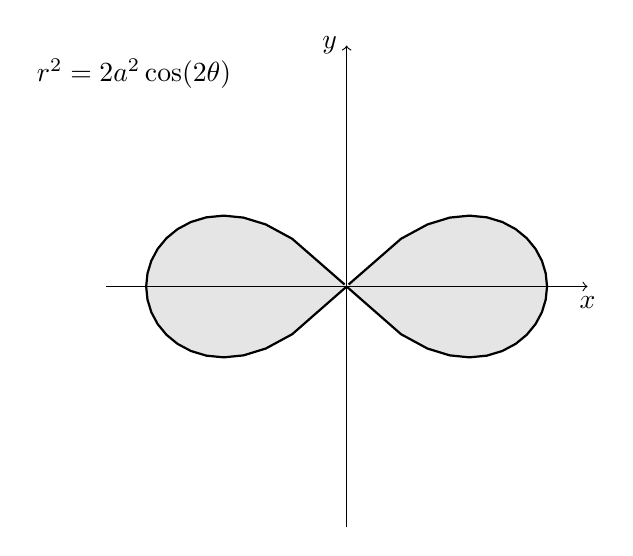
\begin{tikzpicture}[scale=1.8]
    % パラメータ
    \def\a{1}

    % 領域を塗りつぶす
    \fill[gray!20, domain=-pi/4:pi/4, variable=\t]
    plot ({\a*sqrt(2*cos(2*\t r)) * cos(\t r)}, {\a*sqrt(2*cos(2*\t r)) * sin(\t r)})
    -- (0,0) -- cycle;


    \fill[gray!20, domain=-pi/4:pi/4, variable=\t]
    plot ({-\a*sqrt(2*cos(2*\t r)) * cos(-\t r)}, {-\a*sqrt(2*cos(2*\t r)) * sin(-\t r)})
    -- (0,0) -- cycle;

    % 軸の描画
    \draw[->] (-1.7,0) -- (1.7,0) node[below] {$x$};
    \draw[->] (0,-1.7) -- (0,1.7) node[left] {$y$};

    % 方程式の描画
    \draw[black, thick, domain=-pi/4:pi/4, variable=\t]
    plot ({\a*sqrt(2*cos(2*\t r)) * cos(\t r)}, {\a*sqrt(2*cos(2*\t r)) * sin(\t r)});


    \draw[black, thick, domain=-pi/4:pi/4, variable=\t]
    plot ({-\a*sqrt(2*cos(2*\t r)) * cos(-\t r)}, {-\a*sqrt(2*cos(2*\t r)) * sin(-\t r)});


    \node at (-1.5,1.5) {$r^2 = 2a^2 \cos(2\theta)$};
\end{tikzpicture}

\newpage


\section*{p290:4}
\addcontentsline{toc}{section}{\texorpdfstring{p290:4}{p290:4}}

\begin{leftbar}
    求める面積を$S$,求める求める体積を$V$とおくと,
    \begin{align*}
        S & = \frac{1}{2} \int_{0}^{2\pi} r^2 \, d \theta                                                           \\
          & =\frac{1}{2} \int_{0}^{2\pi} a^2 (1+ 2\cos \theta + \cos ^2 \theta) \, d \theta                         \\
          & = \frac{1}{2} \int_{0}^{2\pi} a^2 \left (1+ 2\cos \theta + \frac{1+\cos 2\theta}{2} \right) \, d \theta \\
          & = a^2 \Bigl [ \frac{3}{2} x + 2\sin \theta +\frac{\sin 2 \theta}{4} \Bigl ]_{0}^{2\pi}                  \\
          & = \frac{3 \pi a^2}{2}
    \end{align*}
    となる.
\end{leftbar}

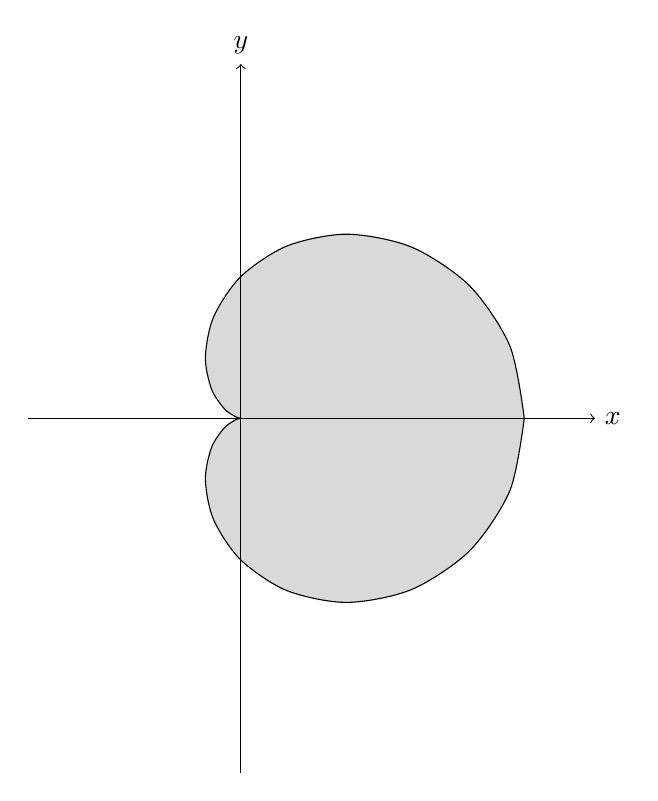
\begin{tikzpicture}[scale=1.8]
    % グレーで塗りつぶす領域の描画
    \fill[gray!30, domain=0:2*pi, variable=\t, smooth]
    plot ({\t r}:{1 + cos(\t r)});

    % r=1+cos(theta)の描画
    \draw[domain=0:2*pi, variable=\t, smooth]
    plot ({\t r}:{1 + cos(\t r)});


    % 軸の描画
    \draw[->] (-1.5,0) -- (2.5,0) node[right] {$x$};
    \draw[->] (0,-2.5) -- (0,2.5) node[above] {$y$};

\end{tikzpicture}

\newpage


\section*{p325--326:1}
\addcontentsline{toc}{section}{\texorpdfstring{p325--326:1}{p325--326:1}}


\subsection*{p325--326:1-(\romannumeral1)}
\addcontentsline{toc}{subsection}{\texorpdfstring{p325--326:1-(\romannumeral1)}{p325--326:1-(\romannumeral1)}}

\begin{tleftbar}
    \[
        I = \int_{-\infty}^{\infty} \frac{dx}{(t+x^2)^{n+1}} \quad (t > 0, n \in \mathbb{N})
    \]

    \[
        (1+x^2)^{n+1} = O(x^{2n+2}) \quad (x \to \pm \infty)
    \]

    \[
        \frac{1}{(t+x^2)^{n+1}} = O(x^{-2n-2}) \quad (x \to \pm \infty)
    \]
    ここで,
    \[
        -2n-2 < -1
    \]
    であるから,定理11.3により,広義積分可能である.

    \[
        x = \sqrt{t} \tan \theta
    \]
    とすると.
    \begin{alignat*}{2}
        I & = \int_{-\frac{\pi}{2}}^{\frac{\pi}{2}} \frac{\cos^{2n+2} \theta}{t^{n+1} } \frac{\sqrt{t}}{\cos^2 \theta} \, d \theta &       &                            \\
          & = \frac{1}{t^{n+1/2}} \int_{-\frac{\pi}{2}}^{\frac{\pi}{2}} \cos^{2n} \theta \, d\theta                                &       &                            \\
          & = \frac{1}{t^{n+1/2}} \int_{0}^{\frac{\pi}{2}} 2 \cos^{2n} \theta \, d\theta                                           &       &                            \\
          & = \frac{1}{t^{n+1/2}} \frac{\Gamma (n+1/2) \Gamma (1/2)}{\Gamma(n+1)}                                                  & \quad & \text{($\because$~定理12.4)} \\
          & = \frac{(2n-1)!! / 2^n \sqrt{\pi} \cdot \sqrt{\pi}}{t^{n+1/2} \cdot (n!)}                                              & \quad & \text{($\because$~定理12.4)} \\\
          & = \frac{(2n-1)!!}{(2n)!!} t^{ - \frac{2n+1}{2}} \pi .
    \end{alignat*}
\end{tleftbar}


\newpage


\subsection*{p325--326:1-(\romannumeral2)}
\addcontentsline{toc}{subsection}{\texorpdfstring{p325--326:1-(\romannumeral2)}{p325--326:1-(\romannumeral2)}}

\begin{tleftbar}
    \[
        F(t) = \int_0^\pi \frac{dx}{(t + \cos x)^2} \quad (t > 1)
    \]

    \[
        f(x,t) = - \frac{1}{t+\cos x} \quad ( 0 \leqq x \leqq \pi , ~ t>1)
    \]
    とすると,
    \[
        \frac{\partial}{\partial t}  f(x,t) = \frac{1}{(t+\cos x)^2}.
    \]
    いま,$f(x,t)$,$\partial f(x,t) / \partial t $は$[0,\pi] \times (1,\infty)$で連続であるから,定理14.1により,
    \begin{align*}
        \frac{\partial}{\partial t} \int_0^\pi f(x,t) \, dx & = \int_0^\pi \frac{\partial}{\partial t} f(x,t) \, dx \\
                                                            & = F(t)
    \end{align*}
    となる.

    また,
    \begin{align*}
        \int_0^\pi f(x,t) \, dx & = \int_0^\pi - \frac{dx}{t+\cos x}                                                        \\
                                & = \int_0^\infty \left ( - \frac{1}{t+\dfrac{1-s^2}{1+s^2}} \right) \frac{2ds}{1+s^2}      \\
                                & = -2\int_0^\infty \frac{ds}{(t-1)s^2+t+1}                                                 \\
                                & = -2 \Bigl [ \frac{1}{\sqrt{t+1}} \arctan \sqrt{\frac{t-1}{t+1}}s \Bigr]_{s=0}^{s=\infty} \\
                                & = \frac{-\pi}{\sqrt{t^2-1}}
    \end{align*}
    より,
    \begin{align*}
        F(t) & = \frac{d}{dt} \frac{-\pi}{\sqrt{t-2-1}}                 \\
             & = \pi \left(-\frac{1}{2} \right) (t^2-1)^{-3/2} \cdot 2t \\
             & = -\frac{\pi t}{(t^2-1)^{3/2}}.
    \end{align*}
\end{tleftbar}
